\part{Behavioral Disease Model}
\label{part:the_model}
\chapter{Model development and justification}
Because the main contribution of this thesis  work  is the presentation of a new multi-system model, the understanding of the reasons that have  lead to its development are important. 
Otherwise the reader can question: "why don't use an already developed and analysed model?
The main answer is that, studying the literature in preparation of the thesis, something missing is noted: the connection between empirical data and epidemiological model. Often a majority of other works relating social and epidemiological aspects read, are pure theoretical models, based on ad-hoc assumptions. Construct a framework based on empirical data related to individual behaviour is challenging \cite{cita24}: untill many years ago, precisely the Coronavirus pamdemic, data on this topic are scarce. The avialbility of research like the one realized by Meta during COVID-19 \cite{cita}, is a major source, both of inspiration and of data for this reason. It permits to explore different behavior related to how people react and deal with the necessity to live with the presence of an infective disease, and it furnish this precious information in a dynamical time series. Often what emerges from this data are non linear dynamic evolution of behavior, while \cite{cita20} many models are based on this technique, this feature is instead taken into account in this work. 
\begin{figure}[h]
	\centering
	\includegraphics[width=0.8\linewidth]{1_corpo/figure/Fig2cut}
	\caption[Mask wearing evolution]{The evolution of mask wearing behaviors.}
	\label{fig:mask_wearing}
\end{figure}
The behavioral-epidemic mean-field models developed want then to interconnect these two features, developing its theoretical framework on empirical evidences, nor on proxy or opinion dataset extrapolate for example by social network, as done for example in \cite{cita2,33}. Not always people opinion correspond to actual behavior, and the fact that this correlation is not necessary and not direct, is another  concept that with the model is attempted to overcome.  
Observing for example the evolution of mask wearing in different European countries, in figure \ref{fig:mask_wearing}. It is immediately visible how at a certain point, there is a net increase in the use of this self-protective device, almost similar to a step. This effect is due to the introduction of regulatory prescription by authorities, and the behavior follows closely the evolution of this stringency. Phenomenon like this, have been considered in the model development, using coefficient parameter, $\psi$ to model the effect of central intervention, and modify the basic persuasion rate of different behaviors. Others empirical evidence on the reasons that undergo the developing of the model can be find in the work \cite{daniele}.

\begin{figure}[h]
	\centering
	\includegraphics[width=0.6\linewidth]{1_corpo/figure/Model_behav_epidemic}
	\caption[Epi-behavior model]{Representation of model with people divided in different behavior and that can have different disease state, untill in the Heedless one that is characterized only by susceptibles.}
	\label{fig:modelbehavepidemic}
\end{figure}


To unveil the model, and initiate its description, first are presented and analysed in the next chapter the two layer that joint together form the entire model: a SIRS epdimemic model, with a Behavior model formed by three compartments: Compliant, Against and Heedless. 
Thre full model is composed by seven compartments, because the heedless behavior is not considered while infected or recovered (because it is quite impossible, unless being completely asymptomatic, act as heedless when infected). The figure \ref{fig:modelbehavepidemic}, describes the population subdivision in a compact form. The infection can be transmitted between all three behaviors, but Compliant group are more cautions, and then a parameter $\rho$ model their reduce probability of being infected, while another $\epsilon$ take consideration of their compliance with self-isolation while infecting, reducing the number of infected compliant ($I_C$ in the model equation) in the mixing that cause new infections in epidemic layer. The behavior are "transmitted" trhough P2P influence, and also a fatigue parameter is considered, to model the drop-out rate due to "fatigue" to mantain a certain behavior. For the epidic model, the classical $\beta$, transmission rate, $\gamma$, recovery rate, and $\delta$, immunity waning rate coefficients are used. 
 



\chapter{Epidemic and Behavioral model alone: a presentation}
\label{ch:model_alone}


To develop a multi-layer system that combines an epidemiological layer with a behavioral one, we first present the dynamics of each layer independently, as presented here. This section briefly introduces the SIRS model, focusing primarily on the reasons for its selection. Then, the Heedless, Compliant, Against behavioral model is introduced, simulated, and analyzed. Understanding the underlying dynamics of this model is crucial for gaining insights into the complex interactions that emerge within the multi-layer structure.


\section{SIRS model}
\label{sec:SIRS}
To describe the epidemic evolution a  SIRS model is implemented. It is an extension of the most famous SIR. Its main addition is the possibility for individuals to become again susceptible after a certain period of time beyond the end of the infection. There are four main characteristic parameters in this model:
\begin{itemize}
	\item $\beta$ is the transmission rate parameter for person-to-person
	contact.
	\item $\gamma$ is the recovery rate.
	\item  $\delta$ is the rate at which immunity recedes following recovery
	\item  $\mathcal{R}(t)$ is the reproduction number, derived as in the $SIR$ model as the ratio between the $\beta$, and $\gamma$ coefficients.
	
\end{itemize}
The choice of an SIR-like model is made because these models are well-known for their ability to describe diseases like COVID-19, and the literature provides numerous examples that use this model \cite{Dehning_2020, Li2022}. The SEIR model could also be a viable choice due to the relevance of the "Exposed" compartment, which effectively captures the disease progression for infections such as COVID-19. In these cases, an incubation period occurs after exposure before symptoms appear and the individual becomes contagious. However, this compartment was excluded because it has been shown \cite{Dehning_2020} that a simpler SIR model can still accurately represent the disease's dynamics. When comparing model simulations with real data, a delay can be incorporated to account for the lag between symptom onset, testing, and reporting. This delay reflects the time needed for symptoms to manifest, conduct testing, and report cases to relevant authorities.

The model includes the possibility of reinfection, which is important when studying long-term scenarios. Considering the effect of individual behavior on disease progression, two critical phases are hypothesized to influence this evolution: the initial stages of the epidemic and the period following the first peak.

In the initial stages, the SIRS model behaves similarly to a typical SIR model because reinfection is unlikely to occur in a short time frame. However, over time, as reinfections become possible, individual attitudes and behaviors will increasingly impact the disease's spread.

\section{Behavioural model}
\label{sec:behavioral_model}

The development of the behavioral model builds on several works already presented in the literature. In particular, the following mechanisms are considered the most relevant:
\begin{itemize}
	\item The competition between two opposing behaviors/opinions, driven by peer pressure \cite{Epstein_2021}.
	\item Non-compliance viewed as a form of social contagion \cite{Bongarti2023}.
	\item The unaware-aware-unaware opinion model class \cite{Zuo2022, Peng2021}.
	\item The fatigue mechanism, where maintaining a certain behavior leads to a spontaneous loss of compliance \cite{Epstein_2021}.
\end{itemize}

To integrate all these aspects into a mean-field model, the first step is to define the compartments used to segment the population. The population is divided into three compartments: Heedless, Compliant, and Against, denoted respectively as H, C, and A. The meaning of each compartment is as follows:
\begin{itemize}
	\item[\textbf{$H$:}] Individuals who behave without much regard for guidelines and are careless about the risks associated with the infection.
	\item[\textbf{$C$:}] Individuals who actively seek to avoid infection or spreading the virus by following guidelines and taking precautions.
	\item[\textbf{$A$:}]Individuals who do not consider the infection a risk to their safety and do not use protection or modify their behavior during the epidemic. They disregard risk-mitigating guidelines and do not align with safer behaviors as the epidemic unfolds.
\end{itemize}

\subsubsection{Initial conditions}
As an initial condition, the hypothesis is that, at the start of the simulation, most of the population is in the Heedless compartment. This assumption is based on the idea that when a new disease emerges, it is poorly understood, and the population has limited information about it. The hypothesis is that people in the Heedless compartment may be clueless about the risks of becoming infected. This lack of knowledge causes them to maintain their usual behavior, making them susceptible to infection. This assumption is also supported by data and literature \cite{Usher_2020}. As an example of this initial configuration, the case of COVID-19 in Italy is considered. In the early stages of its spread, when the disease was primarily affecting China, it was not viewed as a significant threat by much of the population in Western countries. It was perceived as a distant issue affecting a faraway nation. Therefore, when the epidemic reached Europe and Italy, both the population and government were caught off guard. There was an initial delay in the implementation of countermeasures, as well as in the dissemination of reliable information about the disease's progression to the general public.

There are two opposing behavioral groups, which in the initial phase of the model comprise a small fraction of the population: Compliant and Against.

The Compliant group actively seeks to reduce their chances of becoming infected. They practice self-protection measures like wearing face masks, sanitizing their hands, and voluntarily limiting their presence in public spaces to reduce contact with others.

In contrast, the Against group consists of individuals who, for personal reasons—such as anti-scientific beliefs, low trust in policymakers, or other concerns—do not take action to minimize their chances of infection or the possibility of infecting others. This category encompasses phenomena such as: 
\begin{itemize} 
	\item vaccine denialism; 
	\item misinformation spread; 
	\item denial of the existence of the disease; 
	\item distrust of doctors and government policies. 
\end{itemize}

The inclusion of the Against compartment stems from the fact that, especially in the early stages of a new disease outbreak, there is often a lack of reliable knowledge. As documented by \cite{McCormack_2020}, this can lead to the spread of false beliefs in the population. It has also been demonstrated \cite{owid-vaccine-skepticism} that misinformation, especially when associated with fear, can have lasting effects. A notable example is the belief that the measles, mumps, and rubella (MMR) vaccine can cause developmental disorders in children. Despite the fact that the original publication making this claim has been scientifically discredited \cite{wakefield1998retracted}, this idea remains popular and has contributed to a rise in vaccine skepticism \cite{owid-vaccine-skepticism}.

\subsubsection{Social contagion dynamic}
The evolution of the model is governed by two principal mechanisms: \begin{itemize} 
	\item Heedless individuals transitioning to either Compliant or Against compartments. 
	\item Compliant and Against individuals returning to the Heedless compartment. 
\end{itemize}
\begin{figure}[h]
	\centering
	\includegraphics[width=0.72\linewidth]{1_corpo/figure/behavior_model_figure}
	\caption[Behavior model]{The figure represents the behavioral model developed, featuring three compartments: Heedless, Compliant, and Against, abbreviated as H, C, and A. The arrows indicate the inflows and outflows between these compartments.}
	\label{fig:behaviormodelfigure}
\end{figure}
The first mechanism is driven by peer pressure: the size of each group and the level of "persuasion" are the parameters that govern this process. It is mathematically modeled similarly to person-to-person disease transmission, as seen in the SIR-like mean-field model described in section \ref{subsubsec:p2p_transmission}. Instead, the return to the Heedless compartment is modeled as a "spontaneous decay" process: individuals naturally leave the Compliant and Against compartments and return to Heedless, transitioning spontaneously depending on the level of "fatigue" associated with maintaining the behavior.

To describe these transitions, different coefficients are introduced. The $k_1$ and $k_2$ are persuasion rates, while $\lambda_1$ and $\lambda_2$ represent fatigue rates. Their meanings are as follows: \begin{itemize} 
	\item $k_1$: persuasion rate from Heedless to Compliant; 
	\item $k_2$: persuasion rate from Heedless to Against; 
	\item $\lambda_1$: rate of leaving the Compliant behavior due to fatigue; 
	\item $\lambda_2$: rate of leaving the Against behavior due to fatigue. 
\end{itemize}

Finally, the resulting differential equations describing the model's dynamic are:
\begin{equation}
	\label{eq:behavioural_eq}
	\begin{cases}
		\dot{H} = -k_1 H C - k_2 H A + \lambda_1 C + \lambda_2 A \\
		\dot{C} = k_1 H C -  \lambda_1 C \\
		\dot{A} = k_2 H A -  \lambda_2 A\\
	\end{cases}
\end{equation}
Another assumption made to describe the model is the principle of mass conservation, meaning that the relationship $H + C + A = 1$ holds. Additionally, the initial conditions described in the previous section are translated as follows:
\begin{equation}
	\begin{cases}
		H(0) = 1 - C_0 - A_0\\
		C(0) = C_0 > 0\\
		A(0) = A_0 > 0\\
	\end{cases}
\end{equation}

\subsubsection{Behavior conversion number}

To simplify the understanding of the system's underlying dynamics, an analogy can be drawn with the reproduction number in epidemic models. By examining the system equations \ref{eq:behavioural_eq}, a relationship can be identified. From both the second and third equations, we can isolate the two coefficients (specifically $k_1 , \lambda_1 $, and  $k_2 , \lambda_2 $ and derive a new parameter, called "Behavior Conversion Rate", $\mathcal{B}$. This rate is the result of the ratio between the persuasion rate and the fatigue decay rate, and can be viewed as a measure of the transmission potential of social contagion. The general formula to calculate it is::
\begin{equation}
	\mathcal{B}_i =\frac{ k_i }{\lambda_i}  \qquad \text{with } i = 1, \text{or } 2.
	\label{eq:behave_rate}
\end{equation}
In the model presented here, $\mathcal{B}_1$ represents the Behavior Conversion Rate associated with the Compliant compartment, while $\mathcal{B}_2$, corresponds to the Against compartment. The results of different numerical simulations will now be displayed to demonstrate how the relationship between these two values influences the evolution of social contagion.

\subsection{Model simulation}
To represent different dynamics, four main cases are now presented. The coefficient values have been set appropriately to highlight different interesting situations in which the system can evolve. These cases represent the majority of possible scenarios:

\begin{itemize}
	\item[I] case: $\mathcal{B}_1, \mathcal{B}_2 <1$, $\mathcal{B}_1 >  \mathcal{B}_2$, and $\lambda_1 > \lambda_2$.
	\item[II] case: $\mathcal{B}_1, \mathcal{B}_2 >1$, $\mathcal{B}_1 =  \mathcal{B}_2$, and $\lambda_1 < \lambda_2$.
	\item[III] case: $\mathcal{B}_1, \mathcal{B}_2 >1$, $\mathcal{B}_1 >  \mathcal{B}_2$, and $\lambda_1 = \lambda_2$.
	\item[IV] case: $\mathcal{B}_1, \mathcal{B}_2 >1$ and $\mathcal{B}_1 >  \mathcal{B}_2$, and $\lambda_1 < \lambda_2$.
\end{itemize}

The values $k_1$, and $k_2$ are calculated from the formula of $\mathcal{B}_1$, and $\mathcal{B}_2$.

In Figure \ref{fig:model__behavior_sim_1}, it is evident that when both Behavior conversion numbers are less than one, social contagion does not spread: even though, in this case, the Compliant and Against compartments together represent $60\%$ of the total population at the beginning of the simulation, they clearly tend to zero over time. In contrast, the right panel shows the case where the two $\mathcal{B}$ values are equal and greater than one. To emphasize the importance of the fatigue rate, it is shown that with a lower $\lambda_2$ value than $\lambda_1$, the Against compartment becomes dominant by the end of the simulation. 
\begin{figure}[h]
	\centering
	\subfloat[][\emph{$\mathcal{B}_1, \mathcal{B}_2 <1$, $\mathcal{B}_1 >  \mathcal{B}_2$, and $\lambda_1 > \lambda_2$.}]
	{\includegraphics[width=0.48\linewidth]{1_corpo/figure/behavioural_equilibrium/behavior_B1_B2_less_1}} \quad
	\subfloat[][\emph{$\mathcal{B}_1, \mathcal{B}_2 >1$, $\mathcal{B}_1 =  \mathcal{B}_2$, and $\lambda_1 < \lambda_2$.}]
	{\includegraphics[width=0.48\linewidth]{1_corpo/figure/behavioural_equilibrium/behavior_B1_equal_B2}} \\
	\caption[Behavioural model simulation first]{Behavioural system dynamics first two cases.}
	\label{fig:model__behavior_sim_1}
\end{figure}
\label{subsec:model_behav}
Figure \ref{fig:model__behavior_sim_2} illustrates two other interesting scenarios. On the left, we observe the dynamics when one of the $\mathcal{B}$ values is greater than the other, and both $\lambda$ values are the same. It is straightforward to understand that this dynamic would also occur if, with the same values, the $\lambda$ of the dominant behavior were greater than the other, as a larger $\lambda$ would result in a higher $k$ (persuasion rate). The right panel, however, presents a particularly intriguing situation. Here, a lower $\lambda_1$ compared to $\lambda_2$, combined with $k_2 > k_1$, leads to an initial rapid spread of the Against group, even though $\mathcal{B}_2 < \mathcal{B}_1$! It is only after some time that the system evolves to the final equilibrium, which matches the left scenario's result, as the $\mathcal{B}$ values are the same in both simulations.

\begin{figure}[h]
	\centering
	\subfloat[][\emph{$\mathcal{B}_1, \mathcal{B}_2 >1$, $\mathcal{B}_1 >  \mathcal{B}_2$, and $\lambda_1 = \lambda_2$.}]
	{\includegraphics[width=0.48\linewidth]{1_corpo/figure/behavioural_equilibrium/behavior_B1_mag_B2_k1_mag_k2}} \quad
	\subfloat[][\emph{$\mathcal{B}_1, \mathcal{B}_2 >1$ and $\mathcal{B}_1 >  \mathcal{B}_2$, and $\lambda_1 < \lambda_2$.}]
	{\includegraphics[width=0.48\linewidth]{1_corpo/figure/behavioural_equilibrium/behavior_B1_mag_B2_k2_mag_k1}} \\
		\caption[Behavioural model simulation second]{Behavioural system dynamics second two cases.}
	\label{fig:model__behavior_sim_2}
\end{figure}

\subsubsection{Equilibrium and stability analysis}
To enhance understanding of the system, equilibria are searched and their stability is studied. As observed, the system’s final equilibrium values vary according to parameter values. Specifically, the coefficients were combined to produce two Behavior conversion numbers, $\mathcal{B}_1$ and $\mathcal{B}_2$. One way to identify and visualize the system’s equilibrium for a specific parameter set is through nullclines.
The nullclines are used in an autonomous system of differential equations (DE)  to sketch the phase plane of such a system. In a system of two DEs: 
  
\begin{align}
	\frac{dx}{dt} &= f(x,y) \\
	\frac{dy}{dt} &= g(x,y)
\end{align}

There are two types of nullclines: $x$-nullcline, and $y$-nullcline. The $x$-nullcline is a set of points in the phase plane so that $\frac{dx}{dt} =0$, and graphically can be represented as a set of vectors that go either straight up or down. Instead, the $y$-nullcline is a set of points in which the $\frac{dx}{dt} =0$. In these points the vectors are horizontal, going either to the left or to the right.

The original three equations system, has been reduced, to two equation. These to better visualize nullclines in a two-dimensional graph, and it is possible using the mass conservation assumption, yielding the following relationship: $1=H+C+A$. The first two equations are then rewritten, substituting the $A$ term, resulting in a two-equation system with two unknowns. This reduction from the original system of three equations \ref{eq:behavioural_eq}  results in the following two-equation system:
\[
\begin{cases}
	\dot{H} = -k_1 H C - k_2 (1-H-C) H + \lambda_1 C + \lambda_2 (1-H-C)\\
	\dot{C} = k_1 H C - \lambda_1 C
\end{cases}
\]
To simplify the readability and use a notation more familiar for plotting, the $H, C$ symbols have been substituted with respectively $x, y$. So equations become:
\begin{equation}
\label{eq:system_nullclines}
\begin{cases}
	\dot{x} = -k_1 y x - k_2 (1-y-x) x + \lambda_1 y + \lambda_2 (1-y-x)\\
	\dot{y} = k_1 y x - \lambda_1 y
\end{cases}
\end{equation}
The nullclines lines can be calculated imposing $\dot{x} = 0$ and $\dot{y} = 0$. Solving the system with this condition applied gives the following two equations. For the first nullcline, with $\dot{x} = 0$:

\begin{equation}\\
\label{eq:x_nullcline}
 y = \frac{x(k_2 - k_2 x + \lambda_2) - \lambda_2}{x(k_2 - k_1)+ \lambda_1- \lambda_2}
\end{equation}
and for the second with $\dot{y} = 0$
\[x = \frac{\lambda_1}{k_1} = 1/\mathcal{B}_1 \quad \text{or } y = 0.
\]
%The selection of the correct $\mathcal{B}_i$ to use for the second nullcline depends on the comparison between the two reproductive ratio values. Seeing the result of the simulation, it is understood that the larger value should be chosen, as it represents the behavior that will dominate at equilibrium, while the other behavior will tend toward zero. Only in the case where the $\mathcal{B}_1, \mathcal{B}_2 < 1$ this rule does not hold, because the result of the second nullcline found with the formula is out of the domain of existence (i.e $x > 1$, while the Compliant, $x$ is a value comprised between $[0,1]$.)
The first nullcline existence condition can be calculated, imposing that the denominator must be not equal to zero. The result is
\[ x \neq \frac{\lambda_2-\lambda_1}{k_2 - k_1} \]
This value of $x$ is in the interval $[0,1]$ only if $\lambda_2>\lambda_1$ and $k_2 > k_1$, or $\lambda_2<\lambda_1$ and $k_2 < k_1$. The second nullcline instead, exists always if $k_1 \neq 0$.

\subsubsection{Equilibria of the system}
From the results find for the $y$-nullcline, it is possible to calculate explicitly the equilibrium value,as the intersection point of the two nullclines, from the equation \ref{eq:x_nullcline}. In fact if $x =\frac{\lambda_1}{k_1}$, the value is $y = 1 -\frac{\lambda_1}{k_1}$.
Instead if $y = 0$, two values are found: $x = 1$, and $x = \frac{\lambda_2}{k_2}$.
The three equilibria points, indicated with the letters $A,B$, and $C$ are then:
\begin{itemize}
	\item $A = (\frac{\lambda_1}{k_1}, 1-\frac{\lambda_1}{k_1})$
	\item $B = (1, 0)$
	\item $C = (\frac{\lambda_2}{k_2}, 0)$
\end{itemize}

\subsubsection{Equilibria stability analysis}
To verify the local stability of the equilibrium points, the Routh-Hurwitz criterion is applied, requiring the Jacobian matrix of the system evaluated at each equilibrium. It is deemed locally stable if it meets the following conditions based on the Routh-Hurwitz criterion:
\begin{itemize}
	\item A negative trace of the Jacobian, tr($J$)$< 0$
	\item A positive determinant of the Jacobian, det($J$) $> 0$
\end{itemize}
When these conditions are fulfilled, the equilibrium point satisfies the Routh-Hurwitz criterion, indicating local stability.
The Jacobian of the system \ref{eq:system_nullclines} is
\begin{equation}
	J = \begin{bmatrix}
		-k_1 y -k_2 +k_2 y+2 k_2 x- \lambda_2 & -k_1 x + k_2 x + \lambda_1-\lambda_2 \\
		k_1 y & k_1 x - \lambda_1
	\end{bmatrix}
\end{equation}
The trace of $J$ is
\begin{equation}
	\text{tr}J = -k_1 y -k_2 +k_2y + 2 k_2 x - \lambda_2 -\lambda_1 +k_1 x
\end{equation}
Its determinant is instead
\begin{equation}
	\text{det}J = k_2 \lambda_1 + \lambda_1 \lambda_2 + 2 k_1 k_2 x^2 - k_1 k_2 x - k_1 \lambda_2 x - 2\cdot k_2 \lambda_1 x + k_1 \lambda_2 y - k_2 \lambda_1 y
\end{equation}

For each defined equilibrium point, an analysis is performed using the Routh-Hurwitz (R-H) criterion to deduce stability conditions expressed as relations between coefficients. This provides a simplified relation under which the system tends toward a specific equilibrium configuration. These relations are expressed in general as relationship between the coefficients $k_1, k_2$, and $\lambda_1, \lambda_2$.

%%%%%%%%%%%%%%%%%%%%%%%%%%%%%%%%%%%%%%%%%%%%%%%%%%%%%%%
\textbf{Stability of point $A$:} Considering the point $(\frac{\lambda_1}{k_1}, 1-\frac{\lambda_1}{k_1})$, the trace evaluated with this value is tr$J(A) = - k_1 - k_2 +k_2 \frac{\lambda_1}{k_1} - \lambda_2 + \lambda_1$. The criterium requires this value to be less than zero, and manipulating the terms it becomes: $-k_1 + \frac{\lambda_1}{k_1}( k_1 + k_2) - \lambda_2 < 0$. From this it is obtained the relation:
\[\frac{\lambda_1}{k_1} < \frac{k_1 + \lambda_2}{k_1 + k_2} \]
Instead, the determinant is det$J(A) = k_1 \lambda_1 - \lambda_1 \lambda_2$. Simplifying the $\lambda_2$ the relation $\lambda_1 < k_1$ is found, that can be inverted, meaning $\frac{k_1}{\lambda_1} = B_1 > 1$.
Furthermore, both the conditions must hold to verify the local stability and this relation can be used also within the trace. Due to $\frac{\lambda_1}{k_1} < 1$, it can be assumed the relation on the trace holds certainly if $\frac{k_1 + \lambda_2}{k_1 + k_2} > 1$, and so $k_1 + \lambda_2 > k_1 + k_2$. From this last inequality the relation $\lambda_2 > k_2$ can be derived, from which $B_2 < 1$. However, if the initial assumption was that $ \frac{k_1 }{\lambda_1} > 1$, this results can be extendetd.
In conclusion, point $A$ is certainly locally stable if $B_1 > 1$, and $B_2 < 1$.  
 
%%%%%%%%%%%%%%%%%%%%%%%%%%%%%%%%%%%%%%%%%%%%%%%%%%%%%%%
\textbf{Stability of point $B$:} The second equilibrium has coordinates $(1,0)$. Calculating the Jacobian determinant at this point yields the expression det$J(B)= - k_2 \lambda_1 + \lambda_1 \lambda_2 + k_1 k_2 - k_1 \lambda_2$. By grouping terms and analyzing the inequality necessary to satisfy the Routh-Hurwitz criterion, this simplifies to $k_1 (k_2 - \lambda_2) - \lambda_1(k_2 - \lambda_2) > 0$, which further reduces to $(k_1 - \lambda_1) (k_2 - \lambda_2) >0$.
This inequality is met if both terms in the product are either positive or negative:
\begin{itemize}
	\item Case $I:$ $k_1 > \lambda_1$, and $k_2 > \lambda_2$
	\item Case $II:$ $k_1 < \lambda_1$, and $k_2 < \lambda_2$
\end{itemize}
Evaluating the trace at this point, the result is tr$J(B) = k_2 - \lambda_2 - \lambda_1 + k_1 < 0 $. Rearranging terms gives the condition $k_1 + k_2 < \lambda_1 + \lambda_2$, which is true only under the Case $II$ identified above. 
Thus, it can be concluded that equilibrium point $B$ is locally stable only if $\frac{k_1}{\lambda_1} <1$, and  $\frac{k_2}{\lambda_2} <1$, which correspond to $B1 < 1$, and $B_2 <1$.

%%%%%%%%%%%%%%%%%%%%%%%%%%%%%%%%%%%%%%%%%%%%%%%%%%%%%%%
\textbf{Stability of point $C$:} The coordinates of this point are $(0, \frac{\lambda_2}{k_2})$. The determinant at this value is given by det$J(C) = k_2 \lambda_1 - \lambda_1 \lambda_2 + k_1 \frac{\lambda_2^2}{k_2} - k_1 \lambda_2 > 0 $. Also here, rearranging terms simplifies the inequality to: $k_2 [\lambda_1 -\lambda_1 \frac{\lambda_2}{k_2} + k_1 \frac{\lambda_2^2}{k_2^2} - k_1 \frac{\lambda_2^2}{k_2}] >0$, $ k_2 [\lambda_1 ( 1 -  \frac{\lambda_2}{k_2}) - k_1 \frac{\lambda_2}{k_2} (1 - \frac{\lambda_2}{k_2})] >0$, which further reduces to:

\[
 k_2 [(\lambda_1 - k_1 \frac{\lambda_2}{k_2})(1 - \frac{\lambda_2}{k_2})] >0
\]
To satisfy the inequality bot terms must have the same sign,as in the previous point $B$:
\begin{itemize}
	\item Case $I:$ $\frac{k_2}{\lambda_2} > \frac{k_1}{\lambda_1} $, and $k_2 > \lambda_2$
 	\item Case $II:$ $\frac{k_2}{\lambda_2} < \frac{k_1}{\lambda_1} $, and $k_2 < \lambda_2$
\end{itemize}
The trace value instead corresponds to tr$J(C) = - k_2 + k_2 \frac{\lambda_2}{k_2} + k1 \frac{\lambda_2}{k_2} - \lambda_1 < 0$, leading to inequality 
$ \frac{\lambda_2}{k_2} (k_1 + k_2) < k_2 + \lambda_1 $. It is found the relation:
\[ \frac{\lambda_2}{k_2} < \frac{k_2 +\lambda_1}{k_1 + k_2}.\]
By choosing Case I, we ensure the trace inequality is satisfied. If $k_2 > \lambda_2$, the ratio $\frac{\lambda_2}{k_2}$ is less than one. So, if the right part of inequality is larger than one, the trace condition holds. The expression rewrite in this way is $\frac{k_2 +\lambda_1}{k_1 + k_2} > 1$, $k_2 +\lambda_1 > k_1 + k_2 $, and finally $\lambda_1 > k_1$. But, if the initial assumption was that $ \frac{k_2 }{\lambda_2} > 1$, this results can be extended and concluding, point C is certainly stable if $B_2> B_1$, $B_2 > 1$.  
 
\subsubsection{Equilibrium simulations}

Based on the equilibrium analysis, we now understand how the model behaves with various parameter values. To confirm these results, nullcline plots for the four previously simulated cases are generated, and the different scenarios are examined. Fist, is important to describe what can be visualized in the nullcline plot. The blue curve is the expression found solvind the x-nullcline, and the almost vertical line in the plot correspond to the point of discontinuity of this expression, as discussed before. The green line is instead the y-nullcline, composed of a vertical and horizontal line, representing the two possible solutions. In purple are visualized the three equilibria points. If are stable they are marked with a diamond, will if unstable with a circle.  
\\
%%%%%%%%%%%%%%%%%%

\textbf{I case: }$\mathcal{B}_1, \mathcal{B}_2 <1$, $\mathcal{B}_1 >  \mathcal{B}_2$, and $\lambda_1 > \lambda_2$. \\
If both the Conversion numbers are less than one, there is only one equilibrium in the phase plane, where both Compliant and Against tend toward zero.

In the left figure \ref{fig:r1r2less1dyn}, the nullcline plot shows an intersection between the two nullclines only at the point $(1,0)$. Under this condition, the only equilibrium is at $H = 1$, with both $A$ and $C$ equal to zero. Using the notation from the system equation, this corresponds to $x = 1$ and $y = 0$. Calculating the trace and determinant of the Jacobian at this point yields tr$J(1,0) = -\frac{209}{12000}$ and det$J = \frac{121}{2400000}$. Thus, the equilibrium is locally asymptotically stable, as it satisfies the Routh-Hurwitz condition.

\begin{figure}[h]
	\centering
	\subfloat[][\emph{$\mathcal{B}_1, \mathcal{B}_2 <1$, $\mathcal{B}_1 >  \mathcal{B}_2$, and $\lambda_1 > \lambda_2$.}]
	{\includegraphics[width=0.48\linewidth]{1_corpo/figure/behavioural_equilibrium/Pr_nullcline_B1_B2_less_1}} \quad
	\subfloat[][\emph{$\mathcal{B}_1, \mathcal{B}_2 >1$, $\mathcal{B}_1 =  \mathcal{B}_2$, and $\lambda_1 < \lambda_2$}]
	{\includegraphics[width=0.48\linewidth]{1_corpo/figure/behavioural_equilibrium/Pr_nullcline_B1_B2_equal}} \\
	\caption[Nullclines first figure]{Nullclines plots of the first two situations analyzed.}
	\label{fig:r1r2less1dyn}
\end{figure}
%%%%%%%%%%%%%%%%%%

\textbf{II case: } $\mathcal{B}_1, \mathcal{B}_2 >1$, $\mathcal{B}_1 =  \mathcal{B}_2$, and $\lambda_1 < \lambda_2$.\\
This second situation is the most complex to analyze. Due to the equal value of the two influence processes, the final equilibrium of the compartments cannot be determined solely by the previously established relations but also depends on the initial conditions.

The Heedless compartment can still be determined using the equations from previous cases, and the same value is obtained for both $x = \lambda_1/k_1$ and $x = \lambda_2/k_2$. Thus, the final equilibrium values of $x$ is $\bar{x} = 0.12$. As it can be seen from the system evolution \ref{fig:model__behavior_sim_1}, and nullcline plots \ref{fig:r1r2less1dyn}, at the equilibrium the Against and Compliant groups are formed by a subdivision of the $1 - \bar{x}$ part. This division depends on the initial conditions of the model.
\begin{figure}[h]
	\centering
	\includegraphics[width=0.7\linewidth]{1_corpo/figure/behavioural_equilibrium/Surface_nullcline_B1_equal_B2}
	\caption[Surface nullcline]{The nullcline functions represented as surfaces in a tridimensional space.}
	\label{fig:surfacenullclineb1equalb2}
\end{figure}
Applying the Routh-Hurwitz criterion does not yield information on this equilibrium because the Jacobian determinant equals zero. An explanation for this is that, given the equilibrium alignment of points $A$ and $C$ and the equality of their conversion numbers,

 the influxes and outfluxes between the Compliant and Against compartments balance. Consequently, the system's evolution is influenced by the initial numbers of Compliant and Against individuals, as once the system reaches the equilibrium value of Heedless, it remains in this configuration. Observing the 3D plot \ref{fig:surfacenullclineb1equalb2} of the complete system, with surfaces for $H$ and $C$, one can visualize a slope where an imaginary inertia-free ball would roll until it settles at the $1/B1 = 1/B2$  value.
%%%%%%%%%%%%%%%%%%%%%%%%%%%%


\textbf{III-a case:} $\mathcal{B}_1, \mathcal{B}_2 >1$, $\mathcal{B}_1 >  \mathcal{B}_2$, and $\lambda_1 = \lambda_2$. \\
In this scenario, as shown in Figure \ref{fig:nullcline_B1_mag_B2}, there is an intersection between the two nullclines, at the point $A$ . The equilibrium has coordinates equal to $x_A = \lambda_1/k_1$ and $y_A = 1 - \lambda_1/k_1 $, derived by solving the nullcline expressions as previously described. Both R-H conditions hold: $trJ(\bar{x},\bar{y}) = -23/105$, and $detJ(\bar{x},\bar{y}) = 2/525$, so the solution is locally asymptotically stable and does not depend on the initial conditions.
%%%%%%%%%%%%%%%%%%%%%%%%%%%%
\textbf{III-b case: }$\mathcal{B}_1<1 \mathcal{B}_2 >1$, $\mathcal{B}_1 <  \mathcal{B}_2$.
The system's evolution shows opposite behavior compared to the previous case, with the Compliant compartment tending to zero at equilibrium. The right panel of Figure \ref{fig:nullcline_B1_mag_B2}, shows two intersections in the phase plane at points $B$, and $C$. At both points, $y=0$, but only point $C$ is locally stable, as it satisfies the R-H conditions. The equilibrium point is calculated as $x_C= \lambda_2/k_2$ and $y_C = 0$.  
\begin{figure}[h]
	\centering
	\subfloat[][\emph{ $\mathcal{B}_1, \mathcal{B}_2 >1$, $\mathcal{B}_1 >  \mathcal{B}_2$, and $\lambda_1 = \lambda_2$.}]
	{\includegraphics[width=0.48\linewidth]{1_corpo/figure/behavioural_equilibrium/Pr_nullcline_B1_mag_B2}} \quad
	\subfloat[][\emph{ $\mathcal{B}_1<1, \mathcal{B}_2 >1$ and $\mathcal{B}_2 >  \mathcal{B}_1$.}]
	{\includegraphics[width=0.48\linewidth]{1_corpo/figure/behavioural_equilibrium/Pr_nullcline_B1_less_B2}} \\
	\caption[Nullclines second figure]{Nullclines plots of the second two situations analyzed.}
	\label{fig:nullcline_B1_mag_B2}
\end{figure}

\textbf{IV case: } $\mathcal{B}_1, \mathcal{B}_2 >1$ and $\mathcal{B}_1 >  \mathcal{B}_2$, and $\lambda_1 < \lambda_2$. \\
In this situation, the equilibrium has the same value, of the III-a case, and also the stability condition are verified. However, the nullcline plot is very different, referring to figure \ref{fig:prnullclineb1_mag_b2_lambda}. The phase plane is much more complex: there are two lines and the discontinuity point for the x-nullcline (the blue line), and the trajectory of convergence to the point A, the only locally stable is more complex.  

In fact, looking at the model simulation in picture \ref{fig:model__behavior_sim_2}, the system initially evolve to what seems as a first equilibrium, corresponding to $x_A = \lambda_2/k_2$, $y_A = 0$, but then, and it is confirmed by R-H, this equilibrium is unstable, and so the model continues its evolution after reaching the real locally stable configuration. 
\begin{figure}[h]
	\centering
	\includegraphics[width=0.48\linewidth]{1_corpo/figure/behavioural_equilibrium/Pr_nullcline_B1_mag_B2_lambda2_mag}
	\caption[Nullcline fourth case]{IV case of nullcline simulation. The A point is the locally stable one.}
	\label{fig:prnullclineb1_mag_b2_lambda}
\end{figure}

\subsubsection{Behavioural model experiment}
To better understand all possible scenarios emerging from the behavioral model, a bunch of simulations is conducted. Four vectors are defined, one for each model parameter, and a separate simulation is performed for each parameter combination. During each simulation, the parameter values remain constant. The variation range for each parameter is as follows:
\begin{itemize}
	\item $k_1$ between $0.1$ and $0.99$
	\item $k_2$ between $0.1$ and $0.99$
	\item $\lambda_1$ between $1/2$ and $1/40$ $d^{-1}$
	\item $k_1$ between $1/2$ and $1/40$ $d^{-1}$
\end{itemize}
The resulting $\mathcal{B}_1, \mathcal{B}_2$ have a range spanning between $0.5$, and $29.7$.
These ranges are chosen based on the assumption that the "fatigue" rate realistically spans between two and forty days, a range supported by prior research, such as the study in \cite{Kwasnicka_2016}. For the behavior persuasion rate ($k_1$, $k_2$), both low and high values for transition rates are included. We observe the dynamics across all states, recording key metrics for each simulation, such as the final compartment values, peak values, and the time of peak occurrence. Additionally, for generating the sensitivity plots, the Conversion number derived from the coefficient combinations in equation \eqref{eq:behave_rate} are applied. 
\subsubsection{Heat map Final Equilibrium states}
The first plots \ref{fig:subfig_sensitivity_behavioural} are heat maps about the final value reached by various compartments, varying $\mathcal{B}_1$ and $\mathcal{B}_2$.

\begin{figure}[h]
	\centering
	\subfloat[][\emph{Final Compliant compartment}]
	{\includegraphics[width=.48\textwidth]{1_corpo/figure/behavioural_equilibrium/Final_Compliant_heat_map}} \quad
	\subfloat[][\emph{Final Against compartment}]
	{\includegraphics[width=.48\textwidth]{1_corpo/figure/behavioural_equilibrium/Final_Against_heat_map}} \\
	\subfloat[][\emph{Final Heedless compartment}]
	{\includegraphics[width=.48\textwidth]{1_corpo/figure/behavioural_equilibrium/Final_Heedless_heat_map}}
	\caption[Final Behavioural compartments]{The final value reached at equilibrium by every compartment in the behavioural model.}
	\label{fig:subfig_sensitivity_behavioural}
\end{figure}

In these pictures is clearly visible the threshold effect observed in the stability analysis performed earlier. While one of the reproduction ratios becomes larger than the other, the system equilibrium is composed by the dominant group and a portion of Careless individuals.The greater is the ratio, the  smaller is the size at equilibrium of the Heedless. Considering the left panel in figure \ref{fig:subfig_sensitivity_behavioural}, if the heat map of Compliant is pass through vertically, clearly untill $B_1 > B_2$, at the equilibrium there are still compliant. Then, when $B_1 > B_2$, the compliant abruptly tend to zero. 

Another figure in which this threshold effect can be observed is \ref{fig:subfig_sensitivity_behavioural_r1}.

\begin{figure}[h]
	\centering
	\subfloat[][\emph{Final Compliant compartment}]
	{\includegraphics[width=.48\textwidth]{1_corpo/figure/behavioural_equilibrium/final_compliant_B1}} \quad
	\subfloat[][\emph{Final Against compartment}]
	{\includegraphics[width=.48\textwidth]{1_corpo/figure/behavioural_equilibrium/final_against_B1}} \\
	\subfloat[][\emph{Final Careless compartment}]
	{\includegraphics[width=.48\textwidth]{1_corpo/figure/behavioural_equilibrium/final_heedless_B1}}
	\caption[Final Behavioural compartments varying $B_1$]{The final value reached at equilibrium by every compartment in the behavioural model varying the $R_1$ coefficient w.r.t different $B_2$ values.}
	\label{fig:subfig_sensitivity_behavioural_r1}
\end{figure}
The plots show how, for a fixed values of $\lambda_1$ and $k_2$, change the size at equilibrium of the system, varying the $k_1$ coefficient. To highlight the threshold effect due to the comparison of reproduction rates, on the x-axis is plotted the $\mathcal{B}_1$  coefficient, that can be calculated knowing the value of  $\lambda_1$ and $k_1$. For the same reason, different $\mathcal{B}_2$ situations are represented. 

The threshold effect is clearly visible here as well. When examining the final values for the Compliant and Against compartments, it is evident that once the $\mathcal{B}_1$ reproductive coefficient becomes dominant, the increase in the final size observed in the Compliant compartment results from a decrease in the Careless compartment.

\subsubsection{Heat map of max compartments value}
Additionally, the peak values reached by the Compliant and Against compartments are observed. Figures \ref{fig:max_against}, and \ref{fig:max_against2} illustrate the maximum value reached by the Against compartment.
Two situations are compared: in the first $k_1 \sim k_2$, while in the other the difference between the two parameter is higher. In the first situation, there are visible three possible situations:

\begin{itemize}
	\item $B_2 $ greather than $B_1$, and the max value correspond to the value at Equilibrium. It is the bottom right part of the picture.
	\item $B_2 < B_1$, but $\lambda_2 > \lambda_1$. These cases are located on the diagonal threshold of the heat map, and are the situations in which there is first a peak of A, but then the C is the dominant group at equilibrium
	\item $B_2 < B_1$ and also $\lambda_2 < \lambda_1$. Here there is no peak, and A tends always to zero, or to remain approximately zero, depending on the initial conditions.
\end{itemize}
These three phenomena are visible also in Figure \ref{fig:max_against2}, in the left panel. Both the right panels in the two figures need as a comparison, to highlight the situation in which, havin a larger persuasion rate, the A is always dominant on the other compartment. As a consequence the peak correspond always to the value at equilibrium, and in no case, the C compartment at equilibrium is different to zero. 

 
\begin{figure}[h]
	\centering
	\subfloat[][\emph{Max Against compartment with $k_1 \sim k_2 $}]
	{\includegraphics[width=.48\textwidth, valign= t]{1_corpo/figure/behavioural_equilibrium/max_againste_heatmap_1}} \quad
	\subfloat[][\emph{Max Against compartment with $k_1 < k_2 $}]
	{\includegraphics[width=.48\textwidth, valign= t]{1_corpo/figure/behavioural_equilibrium/max_againste_heatmap_2}} \\
	\caption[Max against first case]{a) The max value of Against varying the $\lambda_1, \lambda_2$. b) The evolution of several Against compartment dynamic, fixing $k_1, \lambda_1$, and $k_2$ and varying only the $\lambda_2$.}
	\label{fig:max_against}
\end{figure}


The first case confirms the dynamics presented earlier in the model simulation in section \ref{subsec:model_behav}. This relationship between the departure rate associated with a certain behavior and the persuasion rate can lead to an initial phase where a behavior not dominant at equilibrium gains traction, reaches a peak, and then gradually declines. In some simulations, this diminishing phase can extend over a significant portion of the simulation time, as illustrated in Figure \ref{fig:model__behavior_sim_2}. The red line, called "section line" in Figure \ref{fig:max_against}, represents the part of the heat map, with the same parameters values used in the simulation of the below figure \ref{fig:max_against2}.

\begin{figure}[h]
	\centering
	\subfloat[][\emph{Against simulation with $k_1 \sim k_2$.}]
	{\includegraphics[width=.48\textwidth]{1_corpo/figure/behavioural_equilibrium/against_evolution_vari_1}} \quad
	\subfloat[][\emph{Against simulation with $k_1< k_2$.}]
	{\includegraphics[width=.48\textwidth]{1_corpo/figure/behavioural_equilibrium/against_evolution_vari_2}} \\
		\caption[Max against first case]{a) The max value of Against varying the $\lambda_1, \lambda_2$. b) The evolution of several Against compartment dynamic, fixing $k_1, \lambda_1$, and $k_2$ and varying only the $\lambda_2$.}
	\label{fig:max_against2}
\end{figure}

\chapter{Behavioral epidemic model}
\label{ch:epi_behav_model}
\section{Model description}

The newly developed model in this thesis, the Susceptible-Against-Heedless-Compliant-Infected-Recovered (SAHCIR) model, combines both epidemic and behavioral components, establishing an innovative approach to disease modeling. This model aims to bridge the epidemiological and social dynamics of an outbreak, integrating empirical observations to compare model outcomes with real-world data, as will be discussed in Chapter \ref{ch:data}. While some existing models combine these aspects, like the one presented in \cite{Bulai2023}, they often rely on predefined assumptions about specific behaviors rather than direct empirical validation.

The SAHCIR  model incorporates a variety of behavioral stances towards safety measures, reflecting both proactive (pro-precaution) and non-compliant (anti-precaution) attitudes. The model also recognizes that, particularly during an epidemic's initial phase, a significant portion of the population may not follow safety measures—not out of skepticism, but due to a lack of awareness about the severity of the outbreak. Additionally, the model allows for government intervention through parameters that influence the spontaneous transition rate from the "Against" to the "Compliant" group, mirroring real-world public health policies aimed at promoting preventive behaviors. 

This model thus provides a more empirically grounded framework for understanding the interplay between public health dynamics and social behaviors, filling a gap in the literature by providing a model designed for direct confrontation with real-world data rather than solely hypothetical scenarios.

%ALTRI ASPETTI INSERITI WRT TO THE BASIC BEHAVIOR MODELthe waning of opinion, lack of interest, after the recovery \cite{Zuo2022,Kemp_2021} The fact that even in the I or R compartments population mantain an against or compliant behviors, not isolate this mechanism only in the S compartments, as done for example in \cite{Zuo2022}. 

The model is composed of two layers coupled together: a disease layer, describing the evolution of an epidemic, and a behaviour layer describing the transition among different behaviours during the epidemic development.
The behavioral layer has three possible compartments, as seen in chapter \ref{sec:behavioral_model}: Heedles, Compliant, and Against.

\begin{itemize}
	\item[$H$:] Heedless, people careless of the risk associated to the infection;
	\item[$C$:] Compliant, composed by person that want avoid to become infected or infect others
	\item[$A$:] Against, who not consider a new infection developing as a risk for its safety and not use protection or change its behaviour during the epidemic. 
\end{itemize}

n this model, behavioral dynamics are combined with a SIRS epidemic framework to create seven distinct, mutually exclusive compartments that capture both disease states and public responses. The Heedless behavior is confined to the first compartment, representing individuals who are susceptible to infection. This reflects the assumption that when a new disease emerges, individuals lack sufficient information to take precautionary actions. Consequently, they behave "normally," without adopting safety measures.

As people transition through stages of infection and recovery, the model assumes they gain awareness of the disease's risks and recognize the importance of infection prevention. Thus, after infection or recovery, it is considered unrealistic for them to remain Heedless. Instead, individuals are divided into two categories: Compliant, those who adopt behaviors to minimize further spread, and Against, who are aware but do not actively prevent transmission, possibly due to personal beliefs or low-risk perception. 

\begin{itemize}
	\item[$S_H$:] Susceptible Heedless, the group where there is the majority of the population at the beginning of an epidemic. There is not much information about disease-associated risk and the people in this compartment have no fear of becoming infected and do not modify their behaviors.
	\item[$S_C$:] Susceptible Compliant, is a group composed of those who want to avoid of becomes infected. People who use non-pharmaceutical interventions to limit the possibility of getting sick.
	\item[$S_A$:] Susceptible Against, the people that refuse the information spread by media or authority. They do not consider the threat represented by the disease and do not respect the safety rules or recommended behavior to avoid getting sick or infecting others. 
	\item[$I_C$:] Infected Compliant, people infected by the virus. In this group go both the $S_C$ and $S_H$ compartments because it is considered that even those who have a "neutral" opinion about the risk associated with the infection, change their minds when become infected. The principal behavior associated with this group is that safety measures such as quarantine are respected, and so a certain part of the infected avoid contact while they are sick.
	\item[$I_A$:] Infected Against, compartment composed by the against became sick. They do not respect self-isolation, and diffuse the disease. 
	\item[$R_C$:] Recovered Compliant, people that are healed from the infection. They cannot be infected, but contribute to raising awareness about the risk associated with the disease. 
	\item[$R_A$:] Recovered Against, the part of the recovered formed by against healed from the infection. The most radicalized can be in this group. They are protected by immunity from a disease in which they don't believe. 
\end{itemize}

The resulting system is described by the following system of differential equations: 
\begin{equation}
	\begin{cases}
		\dot{S_H} = - \psi k_1 S_H \cdot C - k_2 S_H \cdot A + \lambda_1 S_C + \lambda_2 S_A + \delta(1-\phi)R_C - \beta S_H \cdot I\\
		\dot{S_C} = \psi k_1 S_H \cdot C + \delta \phi R_C - \lambda_1 S_C - \beta \rho S_C \cdot I  \\
		\dot{S_A} = k_2 S_H \cdot A - \lambda_2 S_A - \beta S_A \cdot I + \delta R_A \\
		\dot{I_C} = \beta \rho S_C \cdot I + \beta S_H \cdot I + \psi k_3 I_A \cdot C - \lambda_3 I_C -  k_4 I_C \cdot A + \lambda_4 I_A - \gamma I_C\\
		 \dot{I_A} = \beta S_A \cdot I - \psi k_3 I_A \cdot C + \lambda_3 I_C + k_4 I_C \cdot A - \lambda_4 I_A - \gamma I_A\\
		 \dot{R_C} = \gamma I_C - k_6 R_C \cdot A + \lambda_6 R_A + \psi k_5 R_A \cdot C - \lambda_5 R_C - \delta R_C\\
		 \dot{R_A} = \gamma I_A + k_6 R_C \cdot A - \lambda_6 R_A - \psi k_5 R_A \cdot C + \lambda_5 R_C - \delta R_A\\
	\end{cases}
	\label{eq:epi_behavioural_eq}
\end{equation}

where
\begin{itemize}
	\item $A = S_A + I_A + R_A$ is the total fraction of Against individuals.
	\item $C = S_C + I_C + R_C$  is the total fraction of Compliant individuals.
	\item $I = \epsilon \cdot I_C + I_A$ is the fraction of infected people participating into the infection process.
	\item $\psi$ is a parameter that represent an increased (if its value is larger than 1) incentive of transition to Compliant group. It can be regarded as an intervention from an external global agent.
	\item $\phi_n$ it is the  a normalized parameter, used to split the population while re entering in the susceptible class in the Heedless or Compliant group. 
	\item $\rho$ is the protection factor of Compliant people that reduces their risk of becoming infected.
	\item $\beta$ is the infectivity rate associated with the disease.
	\item $\gamma$ is the recovery rate.
	\item $\delta$ is the rate at which immunity waves (so that recovered people become susceptible again).
	\item $\epsilon$ specifies the fraction of compliant infected that participate to the infection process.
\end{itemize}

\begin{figure}[tbph]
	\centering
	\includegraphics[width=0.5\linewidth]{1_corpo/figure/epi_behaviour_model_figure}
	\caption[Epidemic behavior model]{Figure of the epidemic behavior model with its compartment and influxes and out-fluxes.}
	\label{fig:epibehaviourmodelfigure}
\end{figure}

\subsection{Basic reproduction number calculation}
The first analysis that can be performed on the Behavioral Disease model is to estimate its basic reproduction number. It is defined as the spectral radius of the next-generation matrix. Using the method outlined in \cite{van_den_Driessche_2017} and now briefly described this quantity is calculated. To distinguish between this value, that is related to the whole model, and so influnced by both the social and epidemic layer, by the classic epidemic only Reproduction number, it is chosen to identify this quantity with the symbol $E_0$. It is the "Epidemic reproduction number". 
Consider $x = (x_1,x_2,...,x_n)^T$ a vector describing the number of individuals that there are in each compartment. The compartments of infected are $m$, and the relation $m < n$ holds. 
Assume that the system has disease free equilibrium (DFE) state, denoted as $x_0$. The $x_0$ exist and is stable in the absence of the disease, so when the infected compartments have value equal to zero. Furthermore in the DFE the linearized equations for $x_1,x_2,...,x_m$ decouple from the other equations. Thanks to the assumption it is possible to write these $m$ infected equations in the form:
\begin{equation}
\label{eq:next_gen1}
\frac{dx_i}{dt} = \mathcal{F}_i(x) - \mathcal{V}_i(x), \text{ for } i =1,2,...m
\end{equation}
The two terms appearing in equation \ref{eq:next_gen1}, are $\mathcal{F}_i(x)$, the rate of appearance of new infected in the compartments $i$, and $ \mathcal{V}_i(x)$ the rate of other transitions between compartment $i$ and other infected compartments. It is assumed that each function is continously differentiable at least twice in each variable.

To describe the evolution of the system the following notation using matrices is adopted: 
\begin{itemize}
	\item $D$ is a $m \times m$ diagonal matrix; the diagonal elements are the relative susceptibilities of the corresponding susceptible class.
	\item $\Pi$ is a $n \times m$ matrix in which the $(k,j)$ element is the fraction of susceptible in the $j^{th}$ compartment that goes into the $k^{th}$ infective compartment.
	\item $b$ is an n-dimensional row vector of relative
	horizontal transmissions.
	\item $\beta'(s, i,r)$ multiplies the $b$ vector and is a scalar factor representing infectivity. It can be constant or a function of other parameters, such as incidence for example. 
	
	\item $V$ is a $n \times n$ matrix describing the transition between the infected state through death and recovery. 
	\item $g(s, i,r)$ is a continuous function representing the inlet of uninfected through birth or immigration. 
	\item $h(s, i, r)$ is also a function but used for the flow into and out of the recovered compartment because of natural immunity or vaccination.
\end{itemize} 

Following the abstraction described above, a generic disease model is represented by the system:

\begin{equation}
	\begin{cases}
		s' = g(s,i,r) - D s \beta'(s,i,r) b i\\
		i' = \Pi D s \beta'(s,i,r) b i - V i\\
		r' = h(s,i,r) + W i \\		
	\end{cases}
	\label{eq:epi_ro_eq}
\end{equation}

Using the defined matrices, according to \cite{arino2007} the Epidemic reproduction number $E_0$ for the model \eqref{eq:epi_ro_eq} at a disease free equilibrium $(s_0, 0, r_0)$ is given by:
\begin{equation}
E_0 = \beta'(s,i,r) b V^{-1} \Pi D s_0
\label{eq:R_0_eqn}
\end{equation}

The disease-free equilibrium is defined as a locally stable equilibrium of the system in which there is no disease and in the sense that a solution starting close to $(s_0, 0, r_0)$ remains close to this state. 

Considering the system dynamic presented in \eqref{eq:epi_behavioural_eq}, this can be rewritten in the matrix form expressed in  \eqref{eq:epi_ro_eq} as: 

\begin{align*}
\Pi & = 
\begin{bmatrix}
	\rho & 1 & 0 \\
	0 & 0 & 1
\end{bmatrix} &
D & = 
\begin{bmatrix}
	1 & 0 & 0 \\
	0 & 1 & 0\\
	0 & 0 & 1
\end{bmatrix} & 
s & = 
\begin{bmatrix}
	SC \\
	SH\\
	SA 
\end{bmatrix} \\
\\
b & = \begin{bmatrix}
	\epsilon & 1
\end{bmatrix} & 
V & = 
\begin{bmatrix}
	k_4 A + \lambda_3 + \gamma & - \phi k_3  C - \lambda_4\\
	- k_4 A - \lambda_3 & \phi k_3 C + \gamma + \lambda_4
\end{bmatrix} & 
i & = 
\begin{bmatrix}
	IC \\
	IA
\end{bmatrix}
\\
\end{align*}


The resulting $E_0$ find with this method is: 
\begin{equation}
	\begin{split}
	E_0 = \frac{\beta}{\gamma}[ & S A_0 (\frac{(\gamma + \lambda_3+A_0\, k_4)}{\sigma}+\frac{\epsilon (\lambda_4 + C_0\, k_3 \,\psi)}{\sigma}) + S H_0 (\frac{(\lambda_3+A_0\, k_4)}{\sigma}+\frac{ \epsilon (\gamma+\lambda_4 + C_0\, k_3 \,\psi)}{\sigma}) \\
	& + S C_0\, \rho (\frac{( \lambda_3+A_0\, k_4)}{\sigma}+\frac{\beta \epsilon (\gamma+\lambda_4 + C_0\, k_3 \,\psi)}{\sigma})] \\
	\text{where}\\
	\sigma = &  \lambda_3 + \lambda_4 + \gamma + A_0 k_4 + C_0  k_3 \psi
	\end{split}
	\label{eq:roepidemicbehavioural}
\end{equation}


Now are presented different cases create to simulate possible different situation with the model. The objective is to verify its evolution, with different sets of parameter, starting from the equivale value of the resulting Reproduction number. 

\subsubsection{$E_0$ first evaluation and example}

A first evaluation of the $E_0$ is done using equation \eqref{eq:R_0_eqn} and assuming that at the beginning of an epidemic, the majority of the population is in the $SH$ compartment, while SC, SA, and also the A and C groups are close to zero. 
An initial tentative calculation for the value is done using a set of values assigned to the rest of the coefficients in the matrices.
For reference, the following values are used:

\begin{align*}
\beta &= 0.40  &\gamma &= 0.35 & \rho &= 0.65 &  \epsilon &= 0.15 \\
k_1 &= 0.49 & k_2 &= 0.243 & \lambda_1 &= 0.143 & \lambda_2 &= 0.143 \\
SC_0 & = 50/60e6 & SA_0 &= 50/60e6 & C &= A = SC_0 & SH_0 & = 1 - SC_0- SA_0\\ 	
\end{align*}


With these coefficient values, considering separately the epidemic and behavioral layers the basic reproduction values are:
 \begin{align*}
 	R_0 &= \frac{\beta}{\gamma} = 1.1429 \\
 	B_1 & = \frac{k_1}{\lambda_1} =  3.3566  \\
 	B_2 & = \frac{k_2}{\lambda_2} = 1.6993 \\
 \end{align*}
For the other behavioral coefficients it is assumed $k_3 = k_5 = k_1$, and $k_4 = k_6 = k_2$. Also $\lambda_3 = \lambda_5 = \lambda_1$, and  $\lambda_4 = \lambda_6 = \lambda_2$.  
In this situation, an epidemic can spread, in fact $R_0>1$, and looking at the behavior of people the complaints, associated with $B_1$, have a larger influence than the one of the "Against" group.

The epidemic-behaviour reproduction number found using the formula and assuming an initial awareness equal to $0.5$ is 
\[E_0 = 0.3898\]

It is immediately noticed that the Epidemic reproduction number is way below the threshold value of 1. According to the theorem presented in \cite{arino2007} there cannot be the spread of disease if the initial $E_0$ is under this value. A simulation of the system dynamic confirms this situation. Observing figure \ref{fig:infected00_epi_behav} can be seen that the number of infected tends to decrease and goes to zero. Then the majority of the population remains in the Susceptible compartment, splitting into compliant and heedless subgroups. This is due to the strongest attractivity of compliant behavior simulated in this scenario.  

\begin{figure}[ht]
	\centering
	\subfloat[][\emph{Susceptibles compartments}]
	{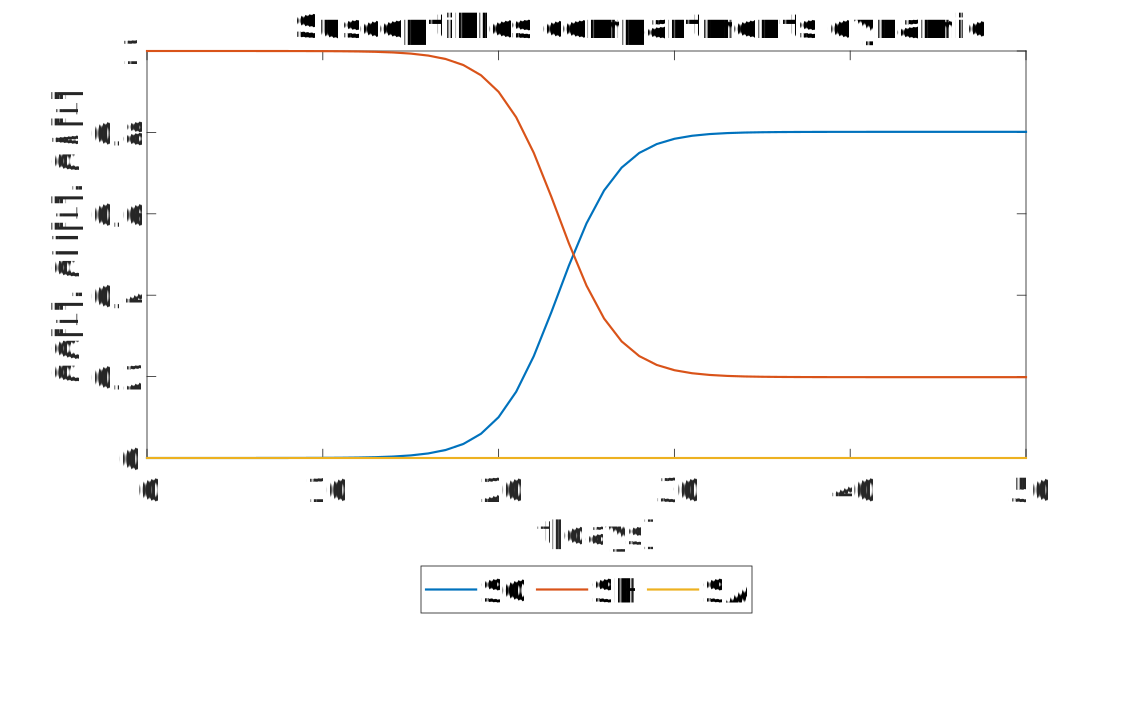
\includegraphics[width=.45\textwidth]{1_corpo/figure/r0/susceptible00_epi_behav}} \quad
	\subfloat[][\emph{Infected compartments}]
	{\includegraphics[width=.45\textwidth]{1_corpo/figure/r0/infected00_epi_behav}} \\
	\subfloat[][\emph{Recovered compartment}]
	{\includegraphics[width=.45\textwidth]{1_corpo/figure/r0/recovered00_epi_behav}}
	\caption[Epidemic behavioral model $R_0$]{Evolution of the behavioral epidemic model, with fixed parameters for the coefficients and an initial reproduction rate less than $1$. It is observed that there aren't conditions for an epidemic to spread.}
	\label{fig:infected00_epi_behav}
\end{figure}

\section{Simulations: how parameters influence the $E_0$ value, and model evolution}

Realize an analysis, as the one done in the previous chapter for the Behavior model alone, is too difficult, because are involved too many equations and parameters. Even if in other articles, as in the work of \cite{Bulai2023}, model similar to the one presented here are analyzed, they used a strong assumption.  Different time scales between the epidemic and behavior layer are hypothesized, and then the analysis performed.

While developing this model, this assumption is not considered reliable. In fact, developing a model that want to use empirical data, this are collected on a daily basis, as the ones about epidemic evolution. For this reason it is considered that the time scales have the same duration.
However, even if this time separation is used for hypothesis, the resulting analysis will produce the same result find with the Behavior model. 

Then, without the possibility of done such analysis, it is important for enhance the understanding of the model, realize extensive experimentation with a series of simulations.
The same four cases parameters, that have been already used in the previous chapter, are used in the behavior layer. For the epidemic layer instead the value is fixed at $R_0 = 3.6$, resulting from supposing a  recovery that last $9$ days, and a transmission rate similar at the one estimated to disease like COVID-19, at the beginning of its diffusion \cite{data_R0_covid}.


\subsection{I case: $\mathcal{B}_1, \mathcal{B}_2 <1$, $\mathcal{B}_1 >  \mathcal{B}_2$, and $\lambda_1 > \lambda_2$}
The first case, is in reality very similar to the one presented, before, and visible in Figure \ref{fig:infected00_epi_behav}. Even in this case an equivalent value of $E_0 = 1.0382$, that is slightly larger than one is found. To appreciate more how the behavior layer evolves here, both the $SC_0$, and $SA_0$ are initialied as equal to the $20 \%$ of the population. Because both the Conversion number are less than one, the majority of the population tend to transition to the Heedleess compartment in this case
\begin{figure}[h]
	\centering
	\subfloat[][\emph{Susceptibles.}]
	{\includegraphics[width=0.48\linewidth]{1_corpo/figure/behav_epi_sim/susceptible_epi_behav_sim_B1_B2_less_1}} \quad
	\subfloat[][\emph{ Infected.}]
	{\includegraphics[width=0.48\linewidth]{1_corpo/figure/behav_epi_sim/infected_epi_behav_sim_B1_B2_less_1}} \\
	\subfloat[][\emph{ Recovered.}]
	{\includegraphics[width=0.48\linewidth]{1_corpo/figure/behav_epi_sim/recovered_epi_behav_sim_B1_B2_less_1}} \quad
	\subfloat[][\emph{ Behavioral model.}]
	{\includegraphics[width=0.48\linewidth]{1_corpo/figure/behav_epi_sim/behavioralepi_behav_sim_B1_B2_less_1}} \\
	\caption[Full model simulation figure first]{Simulations with $\mathcal{B}_1, \mathcal{B}_2 <1$, $\mathcal{B}_1 >  \mathcal{B}_2$, and $\lambda_1 > \lambda_2$.}
	\label{fig:sim_B1_B2_less_1}
\end{figure}





\subsection{II case: $\mathcal{B}_1, \mathcal{B}_2 >1$, $\mathcal{B}_1 =  \mathcal{B}_2$, and $\lambda_1 < \lambda_2$.}
\begin{figure}[hbpt]
	\centering
	\subfloat[][\emph{Susceptibles.}]
	{\includegraphics[width=0.48\linewidth]{1_corpo/figure/behav_epi_sim/susceptible_epi_behav_sim_B1_B2_equal}} \quad
	\subfloat[][\emph{ Infected.}]
	{\includegraphics[width=0.48\linewidth]{1_corpo/figure/behav_epi_sim/infected_epi_behav_sim_B1_B2_equal}} \\
	\subfloat[][\emph{ Recovered.}]
	{\includegraphics[width=0.48\linewidth]{1_corpo/figure/behav_epi_sim/recovered_epi_behav_sim_B1_B2_equal}} \quad
	\subfloat[][\emph{ Behavioral model.}]
	{\includegraphics[width=0.48\linewidth]{1_corpo/figure/behav_epi_sim/behavioralepi_behav_sim_B1_B2_equal}} \\
	\caption[Full model simulation figure first]{Simulations with $\mathcal{B}_1, \mathcal{B}_2 <1$, $\mathcal{B}_1 >  \mathcal{B}_2$, and $\lambda_1 > \lambda_2$.}
	\label{fig:sim_B1_equal_B2}
\end{figure}




\subsection{III bis case: $\mathcal{B}_1, \mathcal{B}_2 >1$, $\mathcal{B}_1 <  \mathcal{B}_2$, and $\lambda_1 = \lambda_2$}

\begin{figure}[h]
	\centering
	\subfloat[][\emph{Susceptibles.}]
	{\includegraphics[width=0.48\linewidth]{1_corpo/figure/behav_epi_sim/susceptible_epi_behav_sim_B1_mag_B2}} \quad
	\subfloat[][\emph{ Infected.}]
	{\includegraphics[width=0.48\linewidth]{1_corpo/figure/behav_epi_sim/infected_epi_behav_sim_B1_mag_B2}} \\
	\subfloat[][\emph{ Recovered.}]
	{\includegraphics[width=0.48\linewidth]{1_corpo/figure/behav_epi_sim/recovered_epi_behav_sim_B1_mag_B2}} \\
	\caption[Full model simulation figure third]{Simulations with $\mathcal{B}_1, \mathcal{B}_2 >1$, $\mathcal{B}_1 >  \mathcal{B}_2$, and $\lambda_1 = \lambda_2$.}
	\label{fig:sim_B2_less_B1}
\end{figure}



\subsection{IV case:  $\mathcal{B}_1, \mathcal{B}_2 >1$ and $\mathcal{B}_1 >  \mathcal{B}_2$, and $\lambda_1 < \lambda_2$}


\begin{figure}[hbpt]
	\centering
	\subfloat[][\emph{Susceptibles.}]
	{\includegraphics[width=0.48\linewidth]{1_corpo/figure/behav_epi_sim/susceptible_epi_behav_sim_B1_mag_B2_lambda2_mag}} \quad
	\subfloat[][\emph{ Infected.}]
	{\includegraphics[width=0.48\linewidth]{1_corpo/figure/behav_epi_sim/infected_epi_behav_sim_B1_mag_B2_lambda2_mag}} \\
	\subfloat[][\emph{ Recovered.}]
	{\includegraphics[width=0.48\linewidth]{1_corpo/figure/behav_epi_sim/recovered_epi_behav_sim_B1_mag_B2_lambda2_mag}} \\
	\caption[Full model simulation figure third]{Simulations with $\mathcal{B}_1, \mathcal{B}_2 >1$ and $\mathcal{B}_1 >  \mathcal{B}_2$, and $\lambda_1 < \lambda_2$.}
	\label{fig:sim_B2_less_B1_lam2}
\end{figure}


\subsection{V case:  $\mathcal{B}_1, \mathcal{B}_2 >1$ and $\mathcal{B}_1 <  \mathcal{B}_2$}


\begin{figure}[h]
	\centering
	\subfloat[][\emph{Susceptibles.}]
	{\includegraphics[width=0.48\linewidth]{1_corpo/figure/behav_epi_sim/susceptible_epi_behav_sim_B2_mag_B1}} \quad
	\subfloat[][\emph{ Infected.}]
	{\includegraphics[width=0.48\linewidth]{1_corpo/figure/behav_epi_sim/infected_epi_behav_sim_B2_mag_B1}} \\
	\subfloat[][\emph{ Recovered.}]
	{\includegraphics[width=0.48\linewidth]{1_corpo/figure/behav_epi_sim/recovered_epi_behav_sim_B2_mag_B1}} 
	\quad
	\subfloat[][\emph{Behavioral full.}]
	{\includegraphics[width=0.48\linewidth]{1_corpo/figure/behav_epi_sim/behavioralepi_behav_sim_B2_mag_B1}} \\
	\caption[Full model simulation figure third]{Simulations with $\mathcal{B}_1, \mathcal{B}_2 >1$ and $\mathcal{B}_1 <  \mathcal{B}_2$.}
	\label{fig:sim_B1_less_B2}
\end{figure}



\begin{figure}[h]
	\centering
	\subfloat[][\emph{$E_0$ with $SA_0, SC_0 \sim 0$.}]
	{\includegraphics[width=0.48\linewidth]{1_corpo/figure/behav_epi_sim/E0_heatmap_1}} \quad
	\subfloat[][\emph{$E_0$ with $SA_0, SC_0 >> 0$.}]
	{\includegraphics[width=0.48\linewidth]{1_corpo/figure/behav_epi_sim/E0_heatmap_2}} \\
	\caption[Heat Map $E_0$]{Heat Map $E_0$, in the case number 5.}
	\label{fig:e0heatmap1}
\end{figure}


\begin{figure}[h]
	\centering
	\subfloat[][\emph{Susceptibles.}]
	{\includegraphics[width=0.48\linewidth]{1_corpo/figure/behav_epi_sim/susceptible_epi_behav_sim_B2_mag_B1_2}} \quad
	\subfloat[][\emph{Infected.}]
	{\includegraphics[width=0.48\linewidth]{1_corpo/figure/behav_epi_sim/infected_epi_behav_sim_B2_mag_B1_2}} \\
	\subfloat[][\emph{ Recovered.}]
	{\includegraphics[width=0.48\linewidth]{1_corpo/figure/behav_epi_sim/recovered_epi_behav_sim_B2_mag_B1_2}} \quad
	\subfloat[][\emph{Behavioral full.}]
	{\includegraphics[width=0.48\linewidth]{1_corpo/figure/behav_epi_sim/behavioralepi_behav_sim_B2_mag_B1_2}} \\
	\caption[Full model simulation figure third]{Simulations with $\mathcal{B}_1, \mathcal{B}_2 >1$ and $\mathcal{B}_1 < \mathcal{B}_2$.}
	\label{fig:sim_B1_less_B2_2}
\end{figure}


